\documentclass[12pt]{beamer}
\usepackage{../Estilos/BeamerMAF}
\usepackage{../Estilos/ColoresLatex}
%Sección para el tema de beamer, con el theme, usercolortheme y sección de footers
\usetheme{CambridgeUS}
\usecolortheme{beaver}
%\useoutertheme{default}
\setbeamercovered{invisible}
% or whatever (possibly just delete it)
\setbeamertemplate{section in toc}[sections numbered]
\setbeamertemplate{subsection in toc}[subsections numbered]
\setbeamertemplate{subsection in toc}{\leavevmode\leftskip=3.2em\rlap{\hskip-2em\inserttocsectionnumber.\inserttocsubsectionnumber}\inserttocsubsection\par}
\setbeamercolor{section in toc}{fg=blue}
\setbeamercolor{subsection in toc}{fg=blue}
\setbeamercolor{frametitle}{fg=blue}
\setbeamertemplate{caption}[numbered]

\setbeamertemplate{footline}
\beamertemplatenavigationsymbolsempty
\setbeamertemplate{headline}{}


\makeatletter
\setbeamercolor{section in foot}{bg=gray!30, fg=black!90!orange}
\setbeamercolor{subsection in foot}{bg=blue!30!yellow, fg=red}
\setbeamercolor{date in foot}{bg=black, fg=white}
\setbeamertemplate{footline}
{
  \leavevmode%
  \hbox{%
  \begin{beamercolorbox}[wd=.333333\paperwidth,ht=2.25ex,dp=1ex,center]{section in foot}%
    \usebeamerfont{section in foot} \insertsection
  \end{beamercolorbox}%
  \begin{beamercolorbox}[wd=.333333\paperwidth,ht=2.25ex,dp=1ex,center]{subsection in foot}%
    \usebeamerfont{subsection in foot}  \insertsubsection
  \end{beamercolorbox}%
  \begin{beamercolorbox}[wd=.333333\paperwidth,ht=2.25ex,dp=1ex,right]{date in head/foot}%
    \usebeamerfont{date in head/foot} \insertshortdate{} \hspace*{2em}
    \insertframenumber{} / \inserttotalframenumber \hspace*{2ex} 
  \end{beamercolorbox}}%
  \vskip0pt%
}
\makeatother\newlength{\depthofsumsign}
\setlength{\depthofsumsign}{\depthof{$\sum$}}
\newcommand{\nsum}[1][1.4]{% only for \displaystyle
    \mathop{%
        \raisebox
            {-#1\depthofsumsign+1\depthofsumsign}
            {\scalebox
                {#1}
                {$\displaystyle\sum$}%
            }
    }
}
\def\scaleint#1{\vcenter{\hbox{\scaleto[3ex]{\displaystyle\int}{#1}}}}
\def\bs{\mkern-12mu}






\AtBeginDocument{\RenewCommandCopy\qty\SI}
\ExplSyntaxOn
\msg_redirect_name:nnn { siunitx } { physics-pkg } { none }
\ExplSyntaxOff

\date{}

\title{\large{Método de Frobenius}}
\subtitle{Tema 2 - Primeras técnicas de solución}
\author{M. en C. Gustavo Contreras Mayén}

\resetcounteronoverlays{saveenumi}

\begin{document}
\maketitle
\fontsize{14}{14}\selectfont
\spanishdecimal{.}

\section*{Contenido}
\frame[allowframebreaks]{\frametitle{Contenido} \tableofcontents[currentsection, hideallsubsections]}


\section{Series de potencias}
\frame[allowframebreaks]{\frametitle{Temas a revisar} \tableofcontents[currentsection, hideothersubsections]}
\subsection{Introducción}

%Ref. Bruzzone - Introducción al método de Frobenius
\begin{frame}
\frametitle{El método de Frobenius}
El método propone la búsqueda de soluciones en series de potencias para ecuaciones diferenciales lineales de segundo orden.
\end{frame}
\begin{frame}
\frametitle{El método de Frobenius}
Este procedimiento requiere el encontrar relaciones de recurrencia entre los coeficientes de las series buscadas, asumiendo un primer término no nulo.
\end{frame}

\subsection{Soluciones analíticas}

\begin{frame}
\frametitle{Soluciones analíticas}
Una clase muy extensa de ecuaciones diferenciales poseen soluciones que se expresan en series de potencias, las cuales son válidas en un dominio determinado.
\\
\bigskip
\pause
Las funciones que gozan de esta particularidad se les llama \textocolor{brown(web)}{analíticas}.
\end{frame}
\begin{frame}
\frametitle{Soluciones analíticas}
Las ecuaciones diferenciales más familiares como la ecuación de un oscilador armónico:
\pause
\begin{align*}
\ddot{x} + \omega^{2} \, x = 0
\end{align*}
\pause
 admite soluciones del tipo:
\pause
\begin{align*}
x (s) = A_{1} \, \sin(\omega \, s) + A_{2} \, \cos (\omega \, s)
\end{align*}
siendo claro que $\sin (\omega \, s)$ y $\cos(\omega \, s)$ son funciones analíticas.
\end{frame}
\begin{frame}
\frametitle{Soluciones analíticas}
De igual manera para la ecuación de un oscilador amortiguado, como en un gran número de ecuaciones de la mecánica nos encontraremos que forman parte de este tipo de ecuaciones.
\end{frame}

\subsection{Definición}

\begin{frame}
\frametitle{Definición de serie de potencias}
Una expresión de la forma:
\pause
\begin{align}
a_{0} + a_{1} \, (x - x_{0}) + \ldots + a_{n} \, x^{n} = \nsum_{n=0}^{\infty} a_{n} \, (x - x_{0})^{n}
\label{eq:ecuacion_01}    
\end{align}
se llama \textocolor{blue-violet}{serie de potencias}.
\end{frame}
\begin{frame}
\frametitle{Límite de la serie}
La serie puede estar definida por el límite:
\pause
\begin{align*}
\lim_{N \to \infty} \nsum_{n=0}^{N} a_{n} \, (x - x_{0})
\end{align*}
para aquellos valores de $x$ en que exista el límite.
\\
\bigskip
\pause
En ese caso, se le conoce a la serie como una \textocolor{byzantine}{serie convergente}.
\end{frame}
\begin{frame}
\frametitle{Criterio de convergencia}
Para determinar los valores de $x$ que cumplen la condición de convergencia, se utiliza el criterio del cociente:
\pause
\begin{align*}
\lim_{n \to \infty} \dfrac{a_{n+1}}{a_{n}} = \rho \hspace{1.5cm} \begin{cases}
\mbox{Converge si } & \rho < 1 \\
\mbox{Diverge si } & \rho > 1
\end{cases}
\end{align*}´
\pause
El criterio no clasifica si $\rho = 1$.
\end{frame}
\begin{frame}
\frametitle{Criterio de convergencia}
Más general es considerar el valor absoluto de dicho cociente, si está acotado por cierto numero $\sigma$ cuando $n \to \infty$, la serie converge cuando $\sigma < 1$.
\end{frame}
\begin{frame}
\frametitle{Criterio de convergencia}
Por lo tanto, tendríamos que:
\pause
\begin{align*}
\rho = \lim_{n \to \infty} \abs{\dfrac{a_{n+1}}{a_{n}}} \, \abs{x - x_{0}} = L \, \abs{x - x_{0}}
\end{align*}
en donde:
\pause
\begin{align*}
L = \lim_{n \to \infty} \abs{\dfrac{a_{n+1}}{a_{n}}}
\end{align*}
\end{frame}
\begin{frame}
\frametitle{Criterio de convergencia}
Si este límite existe, se deduce por la ec. (\ref{eq:ecuacion_01}):
\pause
\begin{align}
\begin{aligned}        
\mbox{converge si } &\abs{x - x_{0}} < \dfrac{1}{L} \\[0.5em]
\mbox{diverge si } &\abs{x - x_{0}} > \dfrac{1}{L}
\end{aligned}
\label{eq:ecuacion_02}    
\end{align}
\end{frame}
\begin{frame}
\frametitle{Intervalo de convergencia}
De esta manera tendremos un intervalo de convergencia cuando $L$ existe:
\pause
\begin{align*}
\left( x_{0} - \dfrac{1}{L}, x_{0} + \dfrac{1}{L} \right)
\end{align*}
\pause
Este intervalo es simétrico respecto de $x_{0}$, de manera tal que \textocolor{ao}{la serie es convergente dentro} de este intervalo y \textocolor{red}{divergente fuera} del mismo.
\end{frame}

\section{Puntos singulares}
\frame[allowframebreaks]{\frametitle{Temas a revisar} \tableofcontents[currentsection, hideothersubsections]}
\subsection{Definiciones}

%Ref. Arfken
\begin{frame}
\frametitle{Definiendo puntos}
Se presenta el concepto de un \textocolor{ao(english)}{punto singular o singularidad} (tal como se aplica a una ecuación diferencial).
\\
\bigskip
\pause
El interés en este concepto radica en su utilidad en:
\pause
\setbeamercolor{item projected}{bg=burgundy,fg=white}
\setbeamertemplate{enumerate items}{%
\usebeamercolor[bg]{item projected}%
\raisebox{1.5pt}{\colorbox{bg}{\color{fg}\footnotesize\insertenumlabel}}%
}
\begin{enumerate}[<+->]
\item Clasificar las EDO.
\item Revisar la viabilidad de una solución en series, esta viabilidad es parte del \textocolor{blue-violet}{teorema de Fuchs}.
\end{enumerate}
\end{frame}
\begin{frame}
\frametitle{Punto ordinario}
Usando la notación $\displaystyle \dv[2]{y}{x} = \sderivada{y}$, tenemos:
\pause
\begin{align}
\sderivada{y} = f (x, y, \pderivada{y})
\label{eq:ecuacion_09_74}
\end{align}
\pause
Ahora bien, si en la ec. (\ref{eq:ecuacion_09_74}) $y$ e $\pderivada{y}$ pueden tener todos los valores finitos a $x = x_{0}$ e $\sderivada{y}$ permanece finita, \pause el punto $x = x_{0}$ es un \textocolor{cadmiumgreen}{punto ordinario}.
\end{frame}
\begin{frame}
\frametitle{Punto singular}
Por otra parte, si $\sderivada{y}$ se vuelve infinita para cualquier selección finita de $y$ e $\pderivada{y}$, \pause el punto $x = x_{0}$ se denomina \textocolor{cardinal}{punto singular}.
\end{frame}
\begin{frame}
\frametitle{Reescribiendo la EDO2}
Si escribimos este EDO2H (en $y$) como:
\pause
\begin{align}
\sderivada{y} + P (x) \: \pderivada{y} + Q (x) \: y = 0
\label{eq:ecuacion_09_75}
\end{align}
\end{frame}
\begin{frame}
\frametitle{Punto singular}
Ahora bien, si las funciones $P (x)$ y $Q (x)$ permanecen finitas a $x = x_{0}$, el punto $x = x_{0}$ es un \textocolor{carnelian}{punto ordinario}.
\\
\bigskip
\pause
Al contrario, si $P (x)$ y/o $Q (x)$ divergen mientras $x \to x_{0}$, el punto $x_{0}$ es un \textocolor{darkcyan}{punto singular}.
\end{frame}
\begin{frame}
\frametitle{Tipos de puntos singulares}
Usando la ecuación (\ref{eq:ecuacion_09_75}) podemos distinguir entre dos tipos de puntos singulares:
\pause
\setbeamercolor{item projected}{bg=citrine,fg=black}
\setbeamertemplate{enumerate items}{%
\usebeamercolor[bg]{item projected}%
\raisebox{1.5pt}{\colorbox{bg}{\color{fg}\footnotesize\insertenumlabel}}%
}
\begin{enumerate}[<+->]
\item Si $P (x)$ y/o $Q (x)$ divergen a medida que $x \to x_{0}$, pero $(x - x_{0}) \: P (x)$ y $(x - x_{0})^{2} \: Q (x)$ permanecen finitas a medida que $x \to x_{0}$,
\seti
\end{enumerate}
\end{frame}
\begin{frame}
\frametitle{Tipos de puntos singulares}
Eentonces el punto $x = x_{0}$ se llama \textocolor{ceruleanblue}{punto singular regular o punto singular no esencial}.
\end{frame}
\begin{frame}
\frametitle{Tipos de puntos singulares}
\setbeamercolor{item projected}{bg=citrine,fg=black}
\setbeamertemplate{enumerate items}{%
\usebeamercolor[bg]{item projected}%
\raisebox{1.5pt}{\colorbox{bg}{\color{fg}\footnotesize\insertenumlabel}}%
}
\begin{enumerate}[<+->]
\conti 
\item Si $P (x)$ diverge más rápidamente que $\dfrac{1}{(x - x_{0})}$, de tal modo que $(x - x_{0}) \: P (x)$ tiene a infinito a medida que $x \to x_{0}$, o cuando $Q (x)$ diverge más rápidamente que $\dfrac{1}{(x - x_{0})^{2}}$, de modo que $(x - x_{0})^{2} \: Q (x)$ tiene a infinito, a medida que $x \to x_{0}$,
\end{enumerate}
\end{frame}
\begin{frame}
\frametitle{Tipos de puntos singulares}
Entonces el punto $x = x_{0}$ se llama \textocolor{darkgreen}{singularidad esencial o singularidad irregular}.
\end{frame}
\begin{frame}
\frametitle{Validez de las definiciones}
Estas definiciones son válidas para todos los valores finitos de $x_{0}$. 
\\
\bigskip
\pause
El análisis de los puntos al infinito $(x \to \infty)$ es similar al tratamiento que se hace para las funciones en variable compleja.
\end{frame}
\begin{frame}
\frametitle{Análisis puntos al infinito}
Hacemos el cambio de variable $x = 1/z$, sustituyendo en la ED y entonces hacemos que $z \to 0$. 
\\
\bigskip
\pause
Haciendo el cambio de variable en las derivadas:
\begin{eqnarray}
\dv{y(x)}{x} = \dv{y(z^{-1})}{z} \: \dv{z}{x} = \pause - \dfrac{1}{x^{2}} \dv{y(z^{-1})}{z} = \pause -z^{2} \: \dv{y(z^{-1})}{z}
\label{eq:ecuacion_09_76}
\end{eqnarray}
\end{frame}
\begin{frame}
\frametitle{Análisis puntos al infinito}
Entonces:
\pause
\begin{eqnarray}
\begin{aligned}
\dv[2]{y(x)}{x} &= \dv{z} \left[ \dv{y(x)}{x} \right] \dv{z}{x} = \\ \pause
&= (-z^{2}) \left[ -2 \: z \dv{y(z^{-1})}{z} - z^{2} \: \dv[2]{y(z^{-1})}{z} \right] = \\ \pause
&= 2 \: z^{3} \: \dv{y(z^{-1})}{z} + z^{4} \: \dv[2]{y(z^{-1})}{z}
\end{aligned}
\label{eq:ecuacion_09_77}
\end{eqnarray}
\end{frame}
\begin{frame}
\frametitle{Análisis puntos al infinito}
Usando estos resultados, podemos transformar la ecuación (\ref{eq:ecuacion_09_75}) en:
\pause
\begin{align}
z^{4} \: \dv[2]{y}{z} + [ 2 \: z^{3} - z^{2} \: P (z^{-1})] \: \dv{y}{z} + Q (z^{-1}) \: y = 0
\label{eq:ecuacion_09_78}
\end{align}
\end{frame}
\begin{frame}
\frametitle{Análisis puntos al infinito}
El comportamiento en $x = \infty, (z = 0)$ entonces dependerá del comportamiento de los nuevos coeficientes:
\pause
\begin{align*}
\dfrac{2 \: z - P(z^{-1})}{z^{2}} \hspace{1cm} \text{ y } \hspace{1cm} \dfrac{Q(z^{-1})}{z^{4}}
\end{align*}
a medida que $z \to 0$.
\end{frame}
\begin{frame}
\frametitle{Análisis puntos al infinito}
Si estas dos expresiones se mantienen finitas, el punto $x = \infty$ es un punto ordinario.
\\
\bigskip
\pause
Si las expresiones divergen con mayor rapidez que $1/z$ y $1/z^{2}$, respectivamente, el punto $x = \infty$ es un punto regular singular, de otra manera, el punto es irregular singular (una singularidad esencial).
\end{frame}

%Ref. Hassani 2009 Chap. 26
\section{Método de Frobenius}
\frame[allowframebreaks]{\frametitle{Temas a revisar} \tableofcontents[currentsection, hideothersubsections]}
\subsection{El método}

\begin{frame}
\frametitle{Descripción del método}
El supuesto básico del método de Frobenius es que la solución de la ED se puede \textocolor{darkred}{representar mediante una serie de potencias}.
\end{frame}
\begin{frame}
\frametitle{Descripción del método}
Esta no es una suposición restrictiva porque todas las funciones encontradas en aplicaciones físicas pueden escribirse como series de potencias siempre que estemos interesados en sus valores que se encuentran en su intervalo de convergencia.
\\
\bigskip
\pause
Este intervalo puede ser muy pequeño o puede cubrir toda la línea real.
\end{frame}
\begin{frame}
\frametitle{La EDO2H general}
Una ecuación diferencial de segundo orden homogénea y lineal, se puede escribir como:
\pause
\begin{align}
p_{2} (x) \, \dv[2]{y}{x} + p_{1} (x) \, \dv{y}{x} + p_{0} (x) \, y = 0
\label{eq:ecuacion_26_07}    
\end{align}
\end{frame}
\begin{frame}
\frametitle{Características de las $p_{i}(x)$}
Para casi todas las aplicaciones que se encuentran en física, consideramos que $p_{0}, p_{1}, p_{2}$ son polinomios.
\\
\bigskip
\pause
Es posible que la ED no se presenta en la forma que se muestra a partir de, digamos, el método de separación de variables, pero se puede \enquote{llevar} a esa forma.
\end{frame}
\begin{frame}
\frametitle{Características de las $p_{i}(x)$}
La forma más complicada de los coeficientes de las derivadas en una ED son típicamente funciones racionales (razones de dos polinomios).
\\
\bigskip
\pause
Por lo tanto, multiplicar la ED por el producto de los tres denominadores nos devolverá la ED en la forma dada en la ec. (\ref{eq:ecuacion_26_07}).
\end{frame}
\begin{frame}
\frametitle{El método de Frobenius}
El primer paso en el método de Frobenius es \textocolor{darksienna}{asumir una serie de potencias infinita para y}.
\\
\bigskip
\pause
Es común elegir que el punto de expansión sea $x = 0$.
\end{frame}
\begin{frame}
\frametitle{El método de Frobenius}
Si $p_{2} (0) \neq 0$, solo es necesario considerar las potencias no negativas de $x$.
\\
\bigskip
\pause
Si $p_{2} (0) = 0$, la ED pierde su carácter de \enquote{segundo orden}, y las soluciones no se revisarían en el curso.
\end{frame}
\begin{frame}
\frametitle{Dos opciones}
Se tienen dos opciones:
\pause
\setbeamercolor{item projected}{bg=darktangerine,fg=black}
\setbeamertemplate{enumerate items}{%
\usebeamercolor[bg]{item projected}%
\raisebox{1.5pt}{\colorbox{bg}{\color{fg}\footnotesize\insertenumlabel}}%
}
\begin{enumerate}[<+->]
\item Elegir un punto de expansión diferente a $x_{0} \neq 0$, tal que $p_{2} (x_{0}) \neq 0$.
\item Permitir las potencias no positivas de $x$ en la expansión de $y$.
\end{enumerate}
\end{frame}
\begin{frame}
\frametitle{Segunda opción}
Rara vez se utiliza la primera opción. Resulta que la forma más económica, pero general, de incorporar la segunda opción es escribir la solución como se muestra a continuación:
\end{frame}
\begin{frame}
\frametitle{Solución supuesta}
La solución que suponemos es del tipo:
\pause
\begin{eqnarray}
\begin{aligned}
y &= x^{r} \, \nsum_{n=0}^{\infty} a_{n} \, x^{n} = \\[0.5em] \pause
&= \nsum_{n=0}^{\infty} a_{n} \, x^{n+r} = \\[0.5em] \pause
&= a_{0} \, x^{r} + a_{1} \, x^{r+1} + a_{2} \, x^{r+2} + \ldots
\end{aligned}
\label{eq:ecuacion_26_08}    
\end{eqnarray}
donde $r$ es un número real (no necesariamente un entero positivo) que quedará determinado por la ED.
\end{frame}
\begin{frame}
\frametitle{El valor de $a_{0}$}
Es habitual elegir $a_{0} = 1$ porque cualquier múltiplo constante de una solución también es una solución.
\\
\bigskip
\pause
Si $a_{0} \neq 1$, entonces se multiplica la serie por $1/a_{0}$ y así obtener el valor.
\end{frame}
\begin{frame}
\frametitle{Característica de la serie}
Ya que una serie de potencias es uniformemente convergente (con su radio de convergencia), por lo que se puede diferenciar término a término.
\end{frame}
\begin{frame}
\frametitle{Diferenciando la solución}
Por lo que al diferenciar la solución en una primera ocasión, tenemos:
\pause
\begin{eqnarray}
\begin{aligned}
\dv{y}{x} &= \nsum_{n=0}^{\infty} a_{n} \, (n + r) \, x^{n+r-1} = \\[0.5em] \pause
&= r \, a_{0} \, x^{r-1} + (r + 1) \, a_{1} \, x^{r} + \ldots
\end{aligned}
\label{eq:ecuacion_26_09a}
\end{eqnarray}
\end{frame}
\begin{frame}
\frametitle{Diferenciando nuevamente la solución}
Por lo que al diferenciar por segunda vez, tenemos:
\pause
\begin{eqnarray}
\begin{aligned}
\dv[2]{y}{x} &= \nsum_{n=0}^{\infty} a_{n} \, (n + r) \, (n + r - 1) \, x^{n+r-2} = \\[0.5em] \pause
&= r \, (r - 1) \, a_{0} \, x^{r-2} + (r + 1) \, r \, a_{1} \, x^{r}-1 + \ldots
\end{aligned}
\label{eq:ecuacion_26_09b}
\end{eqnarray}
\end{frame}
\begin{frame}
\frametitle{Siguiente paso}
Ahora sustituimos las ecuaciones (\ref{eq:ecuacion_26_08}), (\ref{eq:ecuacion_26_09a}) y (\ref{eq:ecuacion_26_09b}) en la ED (\ref{eq:ecuacion_26_07}).
\\
\bigskip
\pause
Multiplicamos los polinomios en la serie, agrupamos todas las potencias distintas de $x$ y establecemos el coeficiente de cada término igual a cero.
\end{frame}
\begin{frame}
\frametitle{Ecuación de índices}
Así obtenemos un conjunto de ecuaciones cuya solución determina el valor de $r$ y las $a_{n}$.
\\
\bigskip
\pause
La ecuación que surge de la \textocolor{darkviolet}{potencia más baja de x} involucra solo a $r$, se llama \textocolor{debianred}{ecuación de índices}.
\end{frame}
\begin{frame}
\frametitle{Ecuación de índices}
Esta suele ser una ecuación cuadrática en $r$ que se puede resolver para obtener el(los) posible(s) valor(es) de $r$, cada uno de los cuales conduce generalmente a una solución diferente.
\end{frame}
\begin{frame}
\frametitle{Ecuación de índices}
Las otras ecuaciones que provienen de potencias superiores de $x$ permiten establecer \textocolor{deeplilac}{relaciones de recurrencia}, es decir, ecuaciones que dan $a_{n}$ en términos de $a_{n-1}$ y $a_{n-2}$.
\\
\bigskip
\pause
Al iterar esta relación, se pueden obtener todos los $a_{n}$ en términos de solo dos coeficientes.
\end{frame}

\subsection{Ejercicio}

%Ref. Zill ED pág. 279
\begin{frame}
\frametitle{Ejercicio práctico}
Resuelve la siguiente EDO2H mediante el método de Frobenius:
\pause
\begin{align}
3 \, x \, \sderivada{y} + \pderivada{y} - y = 0
\label{eq:ecuacion_04}    
\end{align}
\end{frame}
\begin{frame}
\frametitle{Revisión de puntos singulares}
Antes de proponer una solución, se revisa si la EDO tiene puntos singulares regulares o irregulares.
\end{frame}
\begin{frame}
\frametitle{EDO en la forma general}
Llevamos la EDO a la forma general:
\begin{align*}
    \sderivada{y} + \dfrac{1}{3 \, x} \, \pderivada{y} - \dfrac{1}{3 \, x} \, y = 0
\end{align*}
\pause
de donde:
\pause
\begin{align*}
    P (x) = \dfrac{1}{3 \, x} \hspace{1.5cm} Q (x) = -\dfrac{1}{3 \, x}
\end{align*}
\end{frame}
\begin{frame}
\frametitle{Revisión en el caso límite}
Entonces revisamos qué sucede cuando $x \to x_{0}$:
\pause
\begin{eqnarray*}
    \lim_{x \to x_{0}} (x - x_{0}) \, P (x) = \pause \lim_{x \to x_{0}} \dfrac{ \left( x - x_{0} \right)}{3 \, x} = \pause 0 \\[1em]
    \lim_{x \to x_{0}} (x - x_{0})^{2} \, Q (x) = \pause \lim_{x \to x_{0}} - \dfrac{\left( x - x_{0} \right)^{2}}{3 \, x} = \pause 0 
\end{eqnarray*}
\pause
Entonces $x = x_{0}$ es un punto singular regular.
\end{frame}
\begin{frame}
\frametitle{Solución}
Una vez que encontramos que la EDO tiene solo un punto singular en $x = 0$, se propone una solución del tipo:
\pause
\begin{align*}
y = \nsum_{n=0}^{\infty} a_{n} \, x^{n+r}
\end{align*}
\pause
Así se tiene que:
\pause
\begin{eqnarray*}
\begin{aligned}
\pderivada{y} &= \nsum_{n=0}^{\infty} (n + r) \, a_{n} \, x^{n+r-1} \\[0.5em] \pause
\sderivada{y} &= \nsum_{n=0}^{\infty} (n + r) \, (n + r - 1) \, a_{n} \, x^{n+r-2}
\end{aligned}
\end{eqnarray*}
\end{frame}
\begin{frame}
\frametitle{Solución}
De modo que al sustituir en la EDO::
\pause
\begin{align*}
&3 \, x \, \sderivada{y} + \pderivada{y} - y = 3 \, \nsum_{n=0}^{\infty} (n + r) \, (n + r - 1) \, a_{n} \, x^{n+r-1} + \\[0.5em]
&+ \nsum_{n=0}^{\infty} (n + r) \, a_{n} \, x^{n+r-1} - \nsum_{n=0}^{\infty} a_{n} \, x^{n+r} =
\end{align*}
\end{frame}
\begin{frame}
\frametitle{Comenzando con el álgebra}
Factorizamos con respecto a $x^{n+r-1}$:
\pause
\begin{align*}
&= \nsum_{n=0}^{\infty} \left[ 3 \, (n + r) \, (n + r - 1) \, a_{n} + (n + r) \, a_{n} \right] x^{n+r-1} + \\[0.5em]
&- \nsum_{n=0}^{\infty} a_{n} \, x^{n+r} =
\end{align*}
\end{frame}
\begin{frame}
\frametitle{Seguimos con el álgebra}
En la primera suma factorizamos con respecto a $a_{n}$:
\pause
\begin{align*}
&= \nsum_{n=0}^{\infty} (n + r) \, a_{n} \left[ 3 (n + r - 1) + 1 \right] x^{n+r-1} + \\[0.5em]
&- \nsum_{n=0}^{\infty} a_{n} \, x^{n+r} =
\end{align*}
\end{frame}
\begin{frame}
\frametitle{Más álgebra}
Desarrollamos el producto en la primera suma:
\pause
\begin{align*}
&= \nsum_{n=0}^{\infty} (n + r) \, a_{n} \left[ 3 n + 3 r - 3 + 1 \right] x^{n+r-1} + \\[0.5em]
&- \nsum_{n=0}^{\infty} a_{n} \, x^{n+r} =
\end{align*}
\end{frame}
\begin{frame}
\frametitle{Simplificando y más álgebra}
Simplificamos el coeficiente de la primera suma:
\pause
\begin{align*}
&= \nsum_{n=0}^{\infty} (n + r) \left[ 3 n + 3 r - 2 \right] \, a_{n} x^{n+r-1} + \\[0.5em]
&- \nsum_{n=0}^{\infty} a_{n} \, x^{n+r}
\end{align*}
\end{frame}
\begin{frame}
\frametitle{Tomando un término de la primera suma}
Como las sumas no tienen el mismo exponente en $x$, tomamos el primer término de la primera suma, es decir, cuando $n = 0$:
\end{frame}
\begin{frame}
\frametitle{Tomando un término de la primera suma}
\begin{align*}
&= r (3 r - 2) \, a_{0} \, x^{-1} + \\[0.5em] 
&+ \nsum_{n=1}^{\infty} (n + r) \left[ 3 n + 3 r - 2 \right] \, a_{n} x^{n+r-1} + \\[0.5em]
&- \nsum_{n=0}^{\infty} a_{n} \, x^{n+r}
\end{align*}
\end{frame}
\begin{frame}
\frametitle{Factorizando términos}
Factorizamos con respecto a $x^{r}$:
\pause
\begin{align*}
&= x^{r} \, \bigg[ r (3 \, r - 2) \, a_{0} \, x^{-1} +  \\[0.5em]
&+ \nsum_{n=1} (n + r)\,(3 \, n + 3 \, r - 2) \, a_{n} \, x^{n-1} - \nsum_{n=0} a_{n} \, x^{n} \bigg]
\end{align*}
\end{frame}
\begin{frame}
\frametitle{Ajustando el índice en las sumas}
Al haber retirado un término en la primera suma, para poder combinar las sumas, ajustamos el índice en la primera suma, es decir, hacemos $\mathcolor{ao}{k} = n - 1$, por lo que $n = \mathcolor{ao}{k + 1}$, y en la segunda suma hacemos $\mathcolor{ao}{k} = n$:
\end{frame}
\begin{frame}
\frametitle{Recorriendo el índice en una suma}
\begin{align*}
&= x^{r} \, \bigg[ r (3 \, r - 2) \, a_{0} \, x^{-1} +  \\[0.5em]
&+ \underbrace{\nsum_{n=1} (n + r)\,(3 \, n + 3 \, r - 2) \, a_{n} \, x^{n-1}}_{k=n-1} - \underbrace{\nsum_{n=0} a_{n} \, x^{n}}_{k=n} \bigg] =
\end{align*}
\end{frame}
\begin{frame}
\frametitle{Simplificando el valor de $k$}
\begin{align*}
&= x^{r} \, \bigg[ r (3 \, r {-} 2) \, a_{0} \, x^{-1} +  \\[0.5em]
&+ \nsum_{\mathcolor{ao}{k}=0} (\mathcolor{ao}{k {+} 1} {+} r)\,(3 \, \mathcolor{ao}{(k {+} 1)} {+} 3 \, r {-} 2) \, a_{\mathcolor{ao}{k+1}} \, x^{\mathcolor{ao}{k}} + \\[0.5em]
&- \nsum_{\mathcolor{ao}{k}=0} a_{\mathcolor{ao}{k}} \, x^{\mathcolor{ao}{k}} \bigg]
\end{align*}
\end{frame}
\begin{frame}
\frametitle{Resolviendo los coeficientes}
\begin{align*}
&= x^{r} \, \bigg[ r (3 \, r {-} 2) \, a_{0} \, x^{-1} +  \\[0.5em]
&+ \nsum_{k=0} (k {+} 1 {+} r)\,(3 k \, + 3 {+} 3 \, r {-} 2) \, a_{k+1} \, x^{k} + \\[0.5em]
&- \nsum_{k=0} a_{k} \, x^{k} \bigg]
\end{align*}
\end{frame}
\begin{frame}
\frametitle{Resolviendo los coeficientes}
\begin{align*}
&= x^{r} \, \bigg[ r (3 \, r {-} 2) \, a_{0} \, x^{-1} +  \\[0.5em]
&+ \nsum_{k=0} (k {+} 1 {+} r)\,(3 k {+} 3 \, r {+} 1) \, a_{k+1} \, x^{k} + \\[0.5em]
&- \nsum_{k=0} a_{k} \, x^{k} \bigg]
\end{align*}
\end{frame}
\begin{frame}
\frametitle{Sumas con el mismo índice}
Hemos logrado que ambas sumas tengan el mismo índice, y en ambas, tenemos un factor común: $x^{k}$, por lo que podemos nuevamente factorizar con respecto a éste término:
\end{frame}
\begin{frame}
\frametitle{Expresión resultante}
Llegamos entonces a:
\pause
\begin{align*}
&= x^{r} \bigg[ r \, (3 \, r - 2) \, a_{0} \, x^{-1} +  \\[0.5em]
&+ \nsum_{k=0}^{\infty} \bigg\{ (k + r + 1)(3 \, k + 3 \, r + 1) \, a_{k+1} - a_{k} \bigg\} \bigg] \, x^{k} = 0
\end{align*}
\end{frame}
\begin{frame}
\frametitle{Los coeficientes de la suma}
Para que esta expresión sea cero para todo $x$, cada uno de los coeficientes en los corchetes debe ser cero.
\\
\bigskip
\pause
Lo que nos devuelve dos resultados importantes.
\end{frame}
\begin{frame}
\frametitle{Resultados importantes}
Esos resultados son:
\setbeamercolor{item projected}{bg=carmine,fg=white}
\setbeamertemplate{enumerate items}{%
\usebeamercolor[bg]{item projected}%
\raisebox{1.5pt}{\colorbox{bg}{\color{fg}\footnotesize\insertenumlabel}}%
}
\begin{enumerate}
\item Lo consideramos de la expresión con la potencia más pequeña del desarrollo:
\begin{align*}
r \, (3 \, r - 2) \, a_{0} = 0
\end{align*}
que se le conoce como \textocolor{darkred}{ecuación de índices} (en algunos textos se traduce como \textocolor{deeplilac}{ecuación indicial}).
\seti
\end{enumerate}
\end{frame}
\begin{frame}
\frametitle{Resultados importantes}
\setbeamercolor{item projected}{bg=carmine,fg=white}
\setbeamertemplate{enumerate items}{%
\usebeamercolor[bg]{item projected}%
\raisebox{1.5pt}{\colorbox{bg}{\color{fg}\footnotesize\insertenumlabel}}%
}
\begin{enumerate}
\conti
\item El siguente resultado es la \textocolor{indiagreen}{relación de recurrencia}:
\begin{align*}
(k + r + 1)(3 \, k + 3 \, r + 1) \, a_{k+1} - a_{k} = 0
\end{align*}
\end{enumerate}
\end{frame}
\begin{frame}
\frametitle{Relación de recurrencia}
Entonces:
\pause
\begin{align}
\begin{aligned}
a_{k+1} &= \dfrac{a_{k}}{(k + r + 1)(3 \, k + 3 \, r + 1)} \\[0.5em]
\text{con } k &= 0, 1, 2, \ldots
\end{aligned}
\label{eq:ecuacion_07}
\end{align}
\end{frame}
\begin{frame}
\frametitle{Soluciones ec. de índices}
De la ecuación de índices, sabemos desde el inicio que $a_{0} \neq 0$, por lo que:
\pause
\begin{align}
r (3 \, r - 2) = 0
\label{eq:ecuacion_06}
\end{align}
\pause
Que tiene por raíces:
\pause
\begin{align*}
r_{1} = \dfrac{2}{3} \hspace{1.5cm} r_{2} = 0
\end{align*}
\end{frame}
\begin{frame}
\frametitle{Primera raíz}
Ocupamos la primera raíz $r_{1} = 2/3$ en la relación de recurrencia (\ref{eq:ecuacion_07}):
\pause
\begin{align}
a_{k+1} = \dfrac{a_{k}}{(3 \, k + 5)(k + 1)} \hspace{1.5cm} k = 0, 1, 2, \ldots
\label{eq:ecuacion_08}    
\end{align}
\end{frame}
\begin{frame}
\frametitle{Primera raíz}
Entonces:
\pause
\begin{eqnarray*}
a_{1} &=& \dfrac{a_{0}}{5 \cdot 1} \\[0.5em] \pause
a_{2} &=& \dfrac{a_{1}}{8 \cdot 2} = \dfrac{a_{0}}{2! \, 5 \cdot 8} \\[0.5em] \pause
a_{3} &=& \dfrac{a_{2}}{11 \cdot 3} = \dfrac{a_{0}}{3! \, 5 \cdot 8 \cdot 11} \\
\vdots \\[0.5em] \pause
a_{n} &=& \dfrac{a_{0}}{n! \, 5 \cdot 8 \cdot 11 \ldots (3\, n + 2)} \hspace{1cm} n = 1, 2, 3, \ldots
\end{eqnarray*}
\end{frame}
\begin{frame}
\frametitle{Primera solución obtenida}
Hemos obtenido la primera solución $y_{1}$ ocupando la raíz $r_{1}$:
\pause
\begin{align}
y_{1} = a_{0} \, x^{2/3} \left[ 1 + \nsum_{n=1}^{\infty} \dfrac{a_{0}}{n! \, 5 \cdot 8 \cdot 11 \ldots (3\, n + 2)} \, x^{n} \right]
\label{eq:ecuacion_10}    
\end{align}
\end{frame}
\begin{frame}
\frametitle{Segunda raíz}
La segunda raíz de la ecuación de índices: $r_{2} = 0$ nos genera una regla de recurrencia distinta:
\pause
\begin{align}
a_{k+1} = \dfrac{a_{k}}{(k+1)(3 \, k +1)} \hspace{1.5cm} k = 0, 1, 2, \ldots
\label{eq:ecuacion_09}    
\end{align}
\end{frame}
\begin{frame}
\frametitle{Coeficientes}
Los coeficientes que se obtienen son:
\pause
\begin{eqnarray*}
a_{1} &=& \dfrac{a_{0}}{1 \cdot 1} \\[0.5em] \pause
a_{2} &=& \dfrac{a_{1}}{2 \cdot 4} = \dfrac{a_{0}}{2! \, 1 \cdot 4}  \\[0.5em] \pause
a_{3} &=& \dfrac{a_{2}}{3 \cdot 7} = \dfrac{a_{0}}{3! \, 4 \cdot 7}  \\[0.5em]
\vdots \\ \pause
a_{n} &=& \dfrac{a_{0}}{n! \, 1 \cdot 4 \cdot 7 \ldots (3 \, n - 2)} \hspace{1cm} n = 1, 2, 3, \ldots
\end{eqnarray*}
\end{frame}
\begin{frame}
\frametitle{Segunda solución}
La segunda solución que obtenemos es:
\pause
\begin{align}
y_{2} = a_{0} \, x^{0} \left[ 1 + \nsum_{n=1}^{\infty} \dfrac{1}{n! \, 1 \cdot 4 \cdot 7 \ldots (3\, n - 2)} \, x^{n} \right]
\label{eq:ecuacion_11}
\end{align}    
\end{frame}
\begin{frame}
\frametitle{Convergencia de las soluciones}
Se puede demostrar que las soluciones (\ref{eq:ecuacion_10}) y (\ref{eq:ecuacion_11}) convergen ambas para todos los valores finitos de $x$.
\end{frame}
\begin{frame}
\frametitle{Independencia de las series}
También es posible ver que las soluciones no es múltiplo de la otra, por lo que $y_{1} (x)$ y $y_{2} (x)$ son linealmente independientes con respecto a $x$.
\end{frame}
\begin{frame}
\frametitle{Principio de superposición}
Por el principio de superposición, tenemos que:
\pause
\begin{eqnarray*}
\begin{aligned}
y &= C_{1} \, y_{1} (x) + C_{2} \, y_{2} = \\[0.5em] \pause
&= C_{1} \, \left[ x^{2/3} + \nsum_{n=1}^{\infty} \dfrac{a_{0}}{n! \, 5 \cdot 8 \cdot 11 \ldots (3\, n + 2)} \, x^{n} \right] + \\[0.5em]
&+ C_{2} \, \left[ 1 + \nsum_{n=1}^{\infty} \dfrac{1}{n! \, 1 \cdot 4 \cdot 7 \ldots (3\, n - 2)} \, x^{n} \right]
\end{aligned}
\end{eqnarray*}
\end{frame}

\subsection{Casos de las raíces}

\begin{frame}
\frametitle{La ecuación de índices}
Al ocupar el método de Frobenius se pueden presentar tres casos, que corresponden a la naturaleza de las raíces de la ecuación de índices.
\end{frame}
\begin{frame}
\frametitle{La ecuación de índices}
Haremos la suposición que $r_{1}$ y $r_{2}$ son las soluciones \textocolor{indigo(web)}{reales} de la ecuación de índices, que cuando son distintas, $r_{1}$ representa la raíz mayor.
\end{frame}

\subsection*{Caso 1}

\begin{frame}
\frametitle{Caso 1}
\textocolor{lasallegreen}{Las raíces no difieren un entero}. \pause Si $r_{1}$ y $r_{2}$ son distintas, pero no difieren  en un entero, entonces existen dos soluciones linealmente independientes de la ED, cuya forma es:
\pause
\begin{subequations}
\begin{align}
y_{1} &= \nsum_{n=0}^{\infty} a_{n} \, x^{n+r_{1}} \hspace{0.5cm} a_{0} \neq 0 \label{eq:ecuacion_14a} \\[0.5em]
y_{2} &= \nsum_{n=0}^{\infty} b_{n} \, x^{n+r_{2}} \hspace{0.5cm} b_{0} \neq 0 \label{eq:ecuacion_14b}
\end{align}
\end{subequations}
\end{frame}

\subsection*{Caso 2}

\begin{frame}
\frametitle{Caso 2}
\textocolor{lust}{Las raíces difieren en un entero positivo.} \pause Si $r_{1} - r_{2} = N$, donde $N$ es un entero positivo, entonces existe dos soluciones linealmente independientes de la ED, de la forma:
\pause
\begin{subequations}
\begin{align}
y_{1} &= \nsum_{n=0}^{\infty} a_{n} \, x^{n+r_{1}} \hspace{0.5cm} a_{0} \neq 0 \label{eq:ecuacion_20a} \\[0.5em]
y_{2} &= C \, y_{1} (x) \ln x + \nsum_{n=0}^{\infty} b_{n} \, x^{n+r_{2}} \hspace{0.5cm} b_{0} \neq 0 \label{eq:ecuacion_20b}
\end{align}
\end{subequations}
\end{frame}

\subsection*{Caso 3}

\begin{frame}
\frametitle{Caso 3}
\textocolor{oldmauve}{Las raíces son iguales.} \pause Si $r_{1} = r_{2}$, siempre existen dos soluciones linealmente independientes de la ED, de la forma:
\pause
\begin{subequations}
\begin{align}
y_{1} &= \nsum_{n=0}^{\infty} a_{n} \, x^{n+r_{1}} \hspace{0.5cm} a_{0} \neq 0 \label{eq:ecuacion_21a} \\[0.5em]
y_{2} &= y_{1} (x) \ln x + \nsum_{n=0}^{\infty} b_{n} \, x^{n+r_{1}} \hspace{0.5cm} b_{0} \neq 0 \label{eq:ecuacion_21b}
\end{align}
\end{subequations}
\end{frame}

\section{Ejercicios a cuenta}
\frame[allowframebreaks]{\frametitle{Temas a revisar} \tableofcontents[currentsection, hideothersubsections]}
\subsection{Para la Tarea 2}

\begin{frame}
\frametitle{Ejercicios a cuenta}
Determina los puntos singulares de las siguientes ED, clasifica cada punto singular en regular o irregular.
\setbeamercolor{item projected}{bg=bananayellow,fg=ao}
\setbeamertemplate{enumerate items}{%
\usebeamercolor[bg]{item projected}%
\raisebox{1.5pt}{\colorbox{bg}{\color{fg}\footnotesize\insertenumlabel}}%
}
\begin{enumerate}
\item $x^{3} \, \sderivada{y} + 4 \, x^{2} \, \pderivada{y} + 3 \, y = 0$
\item $x \, \sderivada{y} - (x + 3)^{-2} \, y = 0$
\item $(x^{2} - 9)^{2} \, \sderivada{y} + (x + 3) \, \pderivada{y} + 2 \, y = 0$
\item $\sderivada{y} - \dfrac{1}{x} \, \pderivada{y} + \dfrac{1}{(x - 1)^{3}} \, y = 0$
\end{enumerate}
\end{frame}
\begin{frame}
\frametitle{Ejercicios a cuenta}
Resuelve las siguientes ED con el método de Frobenius:
\setbeamercolor{item projected}{bg=lava,fg=white}
\setbeamertemplate{enumerate items}{%
\usebeamercolor[bg]{item projected}%
\raisebox{1.5pt}{\colorbox{bg}{\color{fg}\footnotesize\insertenumlabel}}%
}
\begin{enumerate} 
\item $2 \, x \, \sderivada{y} - \pderivada{y} + 2 \, y = 0$
\item $2 \, x \, \sderivada{y} + 5 \, \pderivada{y} + x \, y = 0$
\item $x (x - 1) \, \sderivada{y} + 3 \, \pderivada{y} - 2 \, y = 0$
\item $\sderivada{y} - \dfrac{3}{x} \, \pderivada{y} - 2 \, y = 0$
\end{enumerate}
\end{frame}

%Ref Kirkwood Chap. 8
\section{Ecuación de calor}
\frame[allowframebreaks]{\frametitle{Temas a revisar} \tableofcontents[currentsection, hideothersubsections]}
\subsection{Problema completo}

\begin{frame}
\frametitle{Ecuación para resolver}
Considera la ecuación de calor:
\pause
\begin{align*}
u_{t} =  \alpha^{2} \,  \laplacian{u}
\end{align*}
La razón por la que las ecuaciones que se obtienen por el método de separación de variables en coordenadas cilíndricas no es tan simple como en coordenadas cartesianas, se debe a la forma del Laplaciano. 
\end{frame}
\begin{frame}
\frametitle{Laplaciano en cilíndricas}
En coordenadas cilíndricas, el laplaciano está dado por:
\pause
\begin{align*}
u_{xx} = u_{rr} + \dfrac{1}{r} \, u_{r} + \dfrac{1}{r^{2}} \, u_{\theta \theta} + u_{zz}
\end{align*}
\end{frame}
\begin{frame}
\frametitle{Primera observación}
Vamos a simplifcar nuestros cálculos y nos permitirá demostrar cómo surgen las funciones de Bessel si suponemos que $u$ es una función de $r$, $\theta$ y $t$, pero no una función de $z$.
\end{frame}

\subsection{Separación de variables}

\begin{frame}
\frametitle{Separación de variables}
Ocupando el método de separación de variables, suponemos que existe una solución para $u$, tal que:
\pause
\begin{align*}
u_{t} = K \, \laplacian{u}
\end{align*}
\end{frame}
\begin{frame}[fragile]
\frametitle{Separación de variables}
Puede expresarse como:
\pause
\begin{align*}
R \, \Theta \, \pderivada{T} = K \, \bigg[ \sderivada{R} \, \Theta \, T + \dfrac{1}{r} \pderivada{R} \, \Theta \, T + \dfrac{1}{r^{2}} \, R \, \sderivada{\Theta} \, T \bigg]
\end{align*}
\end{frame}
\begin{frame}
\frametitle{Acomodando los términos}
Dividiendo entre $K \, R \, \Theta \, T $, tenemos que:
\pause
\begin{align}
\dfrac{1}{K} \, \dfrac{\pderivada{T}}{T} = \dfrac{\sderivada{R}}{R} + \dfrac{1}{r} \, \dfrac{\pderivada{R}}{R} + \dfrac{1}{r^{2}} \, \dfrac{\sderivada{\Theta}}{\Theta}
\label{eq:ecuacion_K01}
\end{align}
\pause
El lado izquierdo de la ecuación es función sólo de $t$.
\end{frame}
\begin{frame}
\frametitle{Separación de variables}
Mientras que el lado derecho de la ecuación es función de $r$ y $\theta$, por lo que deben ser igual a una constante.
\\
\bigskip
\pause
En este caso, corresponde a la primera constante de separación: $- \lambda$.
\end{frame}
\begin{frame}
\frametitle{Ecuaciones resultantes}
Entonces tenemos que:
\pause
\begin{align*}
\dfrac{1}{\alpha^{2}} \, \dfrac{\pderivada{T}}{T} = - \lambda
\end{align*}
o de manera equivalente:
\pause
\begin{align}
\pderivada{T} + \lambda \, K \, T = 0
\label{eq:ecuacion_K02}    
\end{align}
\end{frame}
\begin{frame}
\frametitle{Segunda ecuación}
También tenemos que:
\pause
\begin{align*}
\dfrac{\sderivada{R}}{R} + \dfrac{1}{r} \, \dfrac{\pderivada{R}}{R} + \dfrac{1}{r^{2}} \, \dfrac{\sderivada{\Theta}}{\Theta} = - \lambda
\end{align*}
\pause
Separando nuevamente las funciones:
\pause
\begin{align*}
\dfrac{\sderivada{R}}{R} + \dfrac{1}{r} \, \dfrac{\pderivada{R}}{R} + \lambda = - \dfrac{1}{r^{2}} \, \dfrac{\sderivada{\Theta}}{\Theta}
\end{align*}
\end{frame}
\begin{frame}
\frametitle{Segunda constante de separación}
Así tenemos:
\pause
\begin{align}
r^{2} \left[ \dfrac{\sderivada{R}}{R} + \dfrac{1}{r} \, \dfrac{\pderivada{R}}{R} + \lambda \right] = - \dfrac{\sderivada{\Theta}}{\Theta}
\label{eq:ecuacion_K03}    
\end{align}
El lado izquierdo de esta ecuación es función solo de $r$ y el lado derecho es una función de $\theta$, por lo que debe ser igual a una constante: $\mu$, la segunda constante de separación.
\end{frame}
\begin{frame}
\frametitle{Ecuación con respecto a $\theta$}
\begin{align}
\sderivada{\Theta} + \mu \, \Theta = 0
\label{eq:ecuacion_K04}    
\end{align}
\end{frame}
\begin{frame}
\frametitle{Simplificando la expresión}
Entonces hacemos:
\pause
\begin{align*}
r^{2} \left[ \dfrac{\sderivada{R}}{R} + \dfrac{1}{r} \, \dfrac{\pderivada{R}}{R} + \lambda \right] = \mu
\end{align*}
\pause
Que al acomodar los términos:
\pause
\begin{align*}
\dfrac{\sderivada{R}}{R} + \dfrac{1}{r} \, \dfrac{\pderivada{R}}{R} + \lambda = \dfrac{\mu}{r^{2}}
\end{align*}
\end{frame}
\begin{frame}
\frametitle{Ecuación resultante}
La ecuación a la que llegamos es:
\pause
\begin{align}
\sderivada{R} + \dfrac{1}{r} \, \pderivada{R} + \left( \lambda - \dfrac{\mu}{r^{2}} \right) \, R = 0
\label{eq:ecuacion_K05}    
\end{align}
\end{frame}
\begin{frame}
\frametitle{Solución de la EDO2H}
Por lo tanto, para resolver la ecuación de calor en coordenadas polares, necesitamos resolver las ecuaciones (\ref{eq:ecuacion_K02}), (\ref{eq:ecuacion_K04}) y (\ref{eq:ecuacion_K05}).
\\
\bigskip
\pause
De éstas, solo la ecuación (\ref{eq:ecuacion_K05}) requiere atención adicional.
\end{frame}
\begin{frame}
\frametitle{Ecuación especial}
La ecuación (\ref{eq:ecuacion_K05}) es (como) una \textocolor{palecarmine}{ecuación diferencial de Bessel}, es decir, presenta la forma de la ED de Bessel, que es una ecuación que como veremos más adelante, \pause va a definir un conjunto de ecuaciones diferenciales de la física matemática que nos llevan a un conjunto de \textocolor{prune}{funciones especiales}.
\end{frame}
\begin{frame}
\frametitle{Ecuación especial}
La ecuación que obtuvimos, se presenta cuando usamos el Laplaciano en coordenadas polares o cilíndricas en la ecuación de onda o la ecuación de calor.
\end{frame}
\begin{frame}
\frametitle{Ecuación especial}
Como punto importante hay que señalar que a partir de una ecuación inicial, bajo cierta geometría encontramos una ED resultante, para obtener su solución. Este modo de trabajo lo retomaremos en el Tema 5 - Funciones Especiales.
\end{frame}
\begin{frame}
\frametitle{La ecuación de Laplace}
En la ecuación de Laplace, veremos que la ecuación tiene la forma:
\pause
\begin{align*}
\sderivada{R} + \dfrac{1}{r} \, \pderivada{R} + \left( m^{2} - \dfrac{n^{2}}{r^{2}} \right) \, R = 0
\end{align*}
y tendrá que manejarse de manera diferente.
\end{frame}
\begin{frame}
\frametitle{Caso especial}
Si hubiéramos asumido que la función $u$ también dependía de $z$ y que la solución propuesta fuese:
\pause
\begin{align*}
u (r, \theta, z, t) =  R \, \Theta \, T \, Z
\end{align*}
la ec. (\ref{eq:ecuacion_K05}) todavía habría sido la única EDO complicada que habría surgido.
\end{frame}

\subsection{Solución en series}

\begin{frame}
\frametitle{Resolviendo la ecuación}
La ecuación (\ref{eq:ecuacion_K05}) es una ecuación diferencial tipo Bessel.
\\
\bigskip
\pause
A continuación, definimos una ED de Bessel, demostraremos una solución a tales ecuaciones y luego haremos una transformación que nos permitirá resolver la ecuación anterior
\end{frame}
\begin{frame}
\frametitle{Resolviendo la ecuación}
Dado que esta es una ED de segundo orden, hay dos soluciones pero una no está acotada en $r=0$.
\\
\bigskip
\pause
Debido a consideraciones físicas, esta será una solución inadmisible para nuestros problemas.
\end{frame}
\begin{frame}
\frametitle{Ecuación tipo Bessel}
Una ecuación diferencial de Bessel es una ecuación de la forma:
\pause
\begin{align*}
x^{2} \, \sderivada{y} (x) + x \,\pderivada{y} (x) + (x^{2} - \nu^{2}) \, y (x) = 0 \hspace{1cm} 0 \leq x < \infty
\end{align*}
\pause
El método de solución que usaremos es mediante una serie de potencias.
\end{frame}
\begin{frame}
\frametitle{Revisión de puntos singulares}
Llevamos la ecuación a la forma estándar:
\pause
\begin{align*}
    \sderivada{y} + \dfrac{1}{x} \, \pderivada{y} + \left( 1 - \dfrac{\nu^{2}}{x^{2}} \right) \, y = 0
\end{align*}
con
\begin{align*}
    P (x) = \dfrac{1}{x} \hspace{1.5cm} Q(x) = 1 - \dfrac{\nu^{2}}{x^{2}}
\end{align*}
\end{frame}
\begin{frame}
\frametitle{Revisión de puntos singulares}
Ahora veamos lo qué sucede cuando $x \to x_{0} = 0$:
\pause
\begin{align*}
\lim_{x \to x_{0}} (x - x_{0}) \, P(x) &= \lim_{x \to 0} \left( x \, \dfrac{1}{x} \right) = 1 \\[1em]
\lim_{x \to x_{0}} (x - x_{0})^{2} \, Q(x) &= \lim_{x \to 0} \left[ x^{2} \, \left( 1 - \dfrac{\nu^{2}}{x^{2}} \right) \right] = - \nu^{2}
\end{align*}
\pause
Entonces $x_{0} = 0$ es un punto singular regular.
\end{frame}
\begin{frame}
\frametitle{Solución a la ecuación}
Proponemos una solución de la forma:
\pause
\begin{align*}
y = \nsum_{n=0}^{\infty} \, a_{n} \, x^{n+r}
\end{align*}
Para que la solución esté acotada en $x = 0$, se necesita que $r \geq 0$.
\end{frame}
\begin{frame}
\frametitle{Diferenciando la solución}
Procedemos a diferenciar y agrupamos los términos, así tenemos que:
\pause
\begin{align*}
\pderivada{y} = \nsum_{n=0}^{\infty} \, a_{n} \, (n + r) \, x^{n+r-1}
\end{align*}
\pause
Por lo que:
\pause
\begin{align*}
x \, \pderivada{y} = \nsum_{n=0}^{\infty} \, a_{n} \, (n + r) \, x^{n+r}
\end{align*}
\end{frame}
\begin{frame}
\frametitle{Segunda derivada}
La segunda derivada es:
\pause
\begin{align*}
\sderivada{y} = \nsum_{n=0}^{\infty} \, a_{n} \, (n + r) \, (n + r - 1) \, x^{n+r-2}
\end{align*}
Por tanto:
\pause
\begin{align*}
x^{2} \, \sderivada{y} = \nsum_{n=0}^{\infty} \, a_{n} \, (n + r) \, (n + r - 1) \, x^{n+r}
\end{align*}
\end{frame}
\begin{frame}
\frametitle{Sustitución en la EDO2}
Al sustituir en la ED tipo Bessel, se obtiene:
\pause
\begin{eqnarray*}
\begin{aligned}
&x^{2} \, \sderivada{y} (x) + x \,\pderivada{y} (x) + (x^{2} - \nu^{2}) \, y(x) = \\[0.5em] \pause
&= \nsum_{n=0}^{\infty} \, \bigg[ \left[ a_{n} \, (n + r) (n + r -1) \, x^{n+r} \right] + a_{n} \, (n + r) \, x^{n+r} + \\[0.5em]
&+ \left[ (a_{n} \, x^{n+r+2} ) - \nu^{2} \, a_{n} \, x^{n+r} \right] \bigg] = 0
\end{aligned}
\end{eqnarray*}
\end{frame}
\begin{frame}
\frametitle{Manejo algebraico}
Como nos interesa identificar el coeficiente de la potencia menor de $x$, arreglamos la ecuación anterior para ordenar los coeficientes de menor potencia a los de mayor potencia, como veremos a continuación:
\end{frame}
\begin{frame}
\frametitle{Ecuación ordenada}
{\fontsize{12}{12}\selectfont
\begin{align*}
&a_{0} \bigg[ r (r - 1) + r - \nu^{2} \bigg] \, x^{r} + a_{1} \bigg[ (r + 1) r + (r + 1) - \nu^{2} \bigg] \, x^{r+1} + \\[0.5em]
&+ \nsum_{n=2}^{\infty} \left\{ a_{n} \bigg[ (n + r) \left[ (n + r) - 1 \right] + (n + r) - \nu^{2} \bigg] + a_{n-2} \right\} \, x^{r+n} =
\end{align*}}
En donde vemos que los dos primeros términos los hemos dejado fuera de la suma. Volvemos a reducir la expresión, para obtener:
\end{frame}
\begin{frame}
\frametitle{Ecuación simplificada}
\begin{align*}
&= a_{0} (r^{2} - \nu^{2}) \, x^{r} + a_{1} \bigg[ (r + 1)^{2} - \nu^{2} \bigg] + \\[0.5em]
&+ \nsum_{n=2}^{\infty} \left\{ \bigg[ (n + r)^{2} - \nu^{2} \bigg] \, a_{n} + a_{n-2} \right\} \, x^{r+n} = 0
\end{align*}
\end{frame}
\begin{frame}
\frametitle{Coeficientes nulos}
Recordemos que el coeficiente de cada potencia de $x$ debe de anularse.
\\
\bigskip
\pause
El coeficiente de $x^{r}$ debe ser igual a cero, lo que nos devuelve la ecuación de índices que nos determina el valor de $r$.
\end{frame}
\begin{frame}
\frametitle{Ecuación de índices}
Si $a_{0} \neq 0$, se tiene que:
\pause
\begin{align*}
r^{2} - \nu^{2} = 0
\end{align*}
\pause
Por lo tanto:
\pause
\begin{align*}
r^{2} = \nu^{2}
\end{align*}
\end{frame}
\begin{frame}
\frametitle{El siguiente coeficiente}
Entonces ocurre:
\pause
\begin{align*}
a_{1} \big[ (r + 1)^{2} - \nu^{2} \big] &= a_{1} \big[ (r + 1)^{2} - r^{2} \big] = \\[0.5em]
&= a_{1} \, \big[ 2 \, r + 1 \big] = 0
\end{align*}
\pause
Si la solución está acotada, entonces $r$ debe de ser un valor no negativo, por tanto $a_{1} = 0$.
\end{frame}
\begin{frame}
\frametitle{Regla de recurrencia}
La regla de recurrencia es:
\pause
\begin{align*}
a_{n} \big[ (n + r) \left[ (n + r) - 1 \right] + (n + r) - \nu^{2} \big] + a_{n-2} = 0
\end{align*}
\pause
que de manera equivalente, tenemos:
\pause
\begin{align*}
&a_{n} \big[ (n + r) \left( (n + r) - 1 \right) + (n + r) - \nu^{2} \big] = \\[0.5em]
&= a_{n} \, \big[ (n + r)^{2} - \nu^{2} \big] + a_{n-2} = 0
\end{align*}
\end{frame}
\begin{frame}
\frametitle{Regla de recurrencia}
Al sustituir $\nu$ para $r$:
\pause
\begin{align*}
a_{n} \, \big[ (n + r)^{2} - \nu^{2} \big] = a_{n} \, n \, (n + 2 \, \nu) = - a_{n-2}
\end{align*}
\pause
Es decir:
\pause
\begin{align*}
a_{n} = \dfrac{- a_{n-2}}{n (n + 2 \, \nu)}
\end{align*}
Como $a_{1} = 0$, entonces $a_{k} = 0$ para todo entero impar $k$.
\end{frame}
\begin{frame}
\frametitle{Coeficientes que se mantienen}
Los coeficientes que se mantienen son los $a_{2 k}$, entonces se tiene que:
\pause
\fontsize{12}{12}\selectfont
\begin{eqnarray*}
a_{2} &=& - \dfrac{a_{0}}{2 (2 + 2 \, \nu)} \\[0.5em]\pause
a_{4} &=& - \dfrac{a_{2}}{4 (4 + 2 \, \nu)} = \dfrac{(-1)}{4 (4 + 2 \nu)} \, \dfrac{(-1)a_{0}}{2 (2 + 2 \nu)} \\[0.5em]\pause
a_{6} &=& - \dfrac{a_{4}}{6 (6 + 2 \, \nu)} = - \dfrac{a_{0}}{2^{3} \, (1 \cdot 2 \cdot 3) (3 + \nu)(2 + 2 \nu)(1 + \nu)}\\
&\ldots&
\end{eqnarray*}
\end{frame}
\begin{frame}
\frametitle{Expresión para los coeficientes}
Entonces para el $k$-ésimo coeficiente, tendremos que:
\pause
\begin{align*}
a_{2k} = \dfrac{(-1)^{k} \, a_{0}}{2^{2 k} \, (k!) \, (k + \nu) \, (k - 1 + \nu) \ldots (1 + \nu)}
\end{align*}
\pause
Entonces podemos presentar una solución a la ecuación diferencial de Bessel:
\end{frame}
\begin{frame}
\frametitle{Solución a la ec. de Bessel}
Tenemos que una de las soluciones a la ecuación de Bessel es:
\pause
{\fontsize{12}{12}\selectfont
\begin{align*}
y_{1}(x) = a_{0} \, x^{\nu} \left[ 1 + \nsum_{k=1}^{\infty} \dfrac{(-1)^{k} \, a_{0} \, k}{2^{2 k} \, (k!) \, (k + \nu) \, (k -1 + \nu)\ldots (1 + \nu)} \right]
\end{align*}}
Que es una solución para cualquier valor de $a_{0}$. Hagamos notar que no se han impuesto condiciones de frontera alguna.
\end{frame}
\begin{frame}
\frametitle{Solución a la ec. de Bessel}
La solución obtenida se le conoce como \textocolor{falured}{función de Bessel de primera clase de orden $\nu$}.
\\
\bigskip
\pause
Se le representa como $J_{\nu} (x)$.
\end{frame}
\begin{frame}
\frametitle{Solución a la ec. de Bessel}
Si hacemos lo siguiente (que es una norma común en física matemática):
\pause
\begin{align*}
a_{0} = \dfrac{1}{\nu!} \, 2^{\nu}
\end{align*}
\pause
Se puede expresar $J_{\nu}(x)$ como:
\pause
\begin{align*}
J_{\nu}(x) = \nsum_{k=0}^{\infty} \dfrac{(-1)^{k} \, x^{2k+\nu}}{2^{2k+\nu} \, (k!) \, (k + \nu)!} = 
\end{align*}
\end{frame}
\begin{frame}
\frametitle{Solución a la ec. de Bessel}
Entonces:
\pause
\begin{align*}
J_{\nu}(x)  = \nsum_{k=0}^{\infty} \dfrac{(-1)^{k} \, \left( \frac{x}{2}\right)^{2k+\nu}}{(k!) \, (k + \nu)!}
\end{align*}
Aplicando la prueba del cociente (razón), la serie converge para todos los valores de $x$.
\end{frame}
\begin{frame}
\frametitle{Las funciones de Bessel}
\begin{figure}[H]
    \centering
    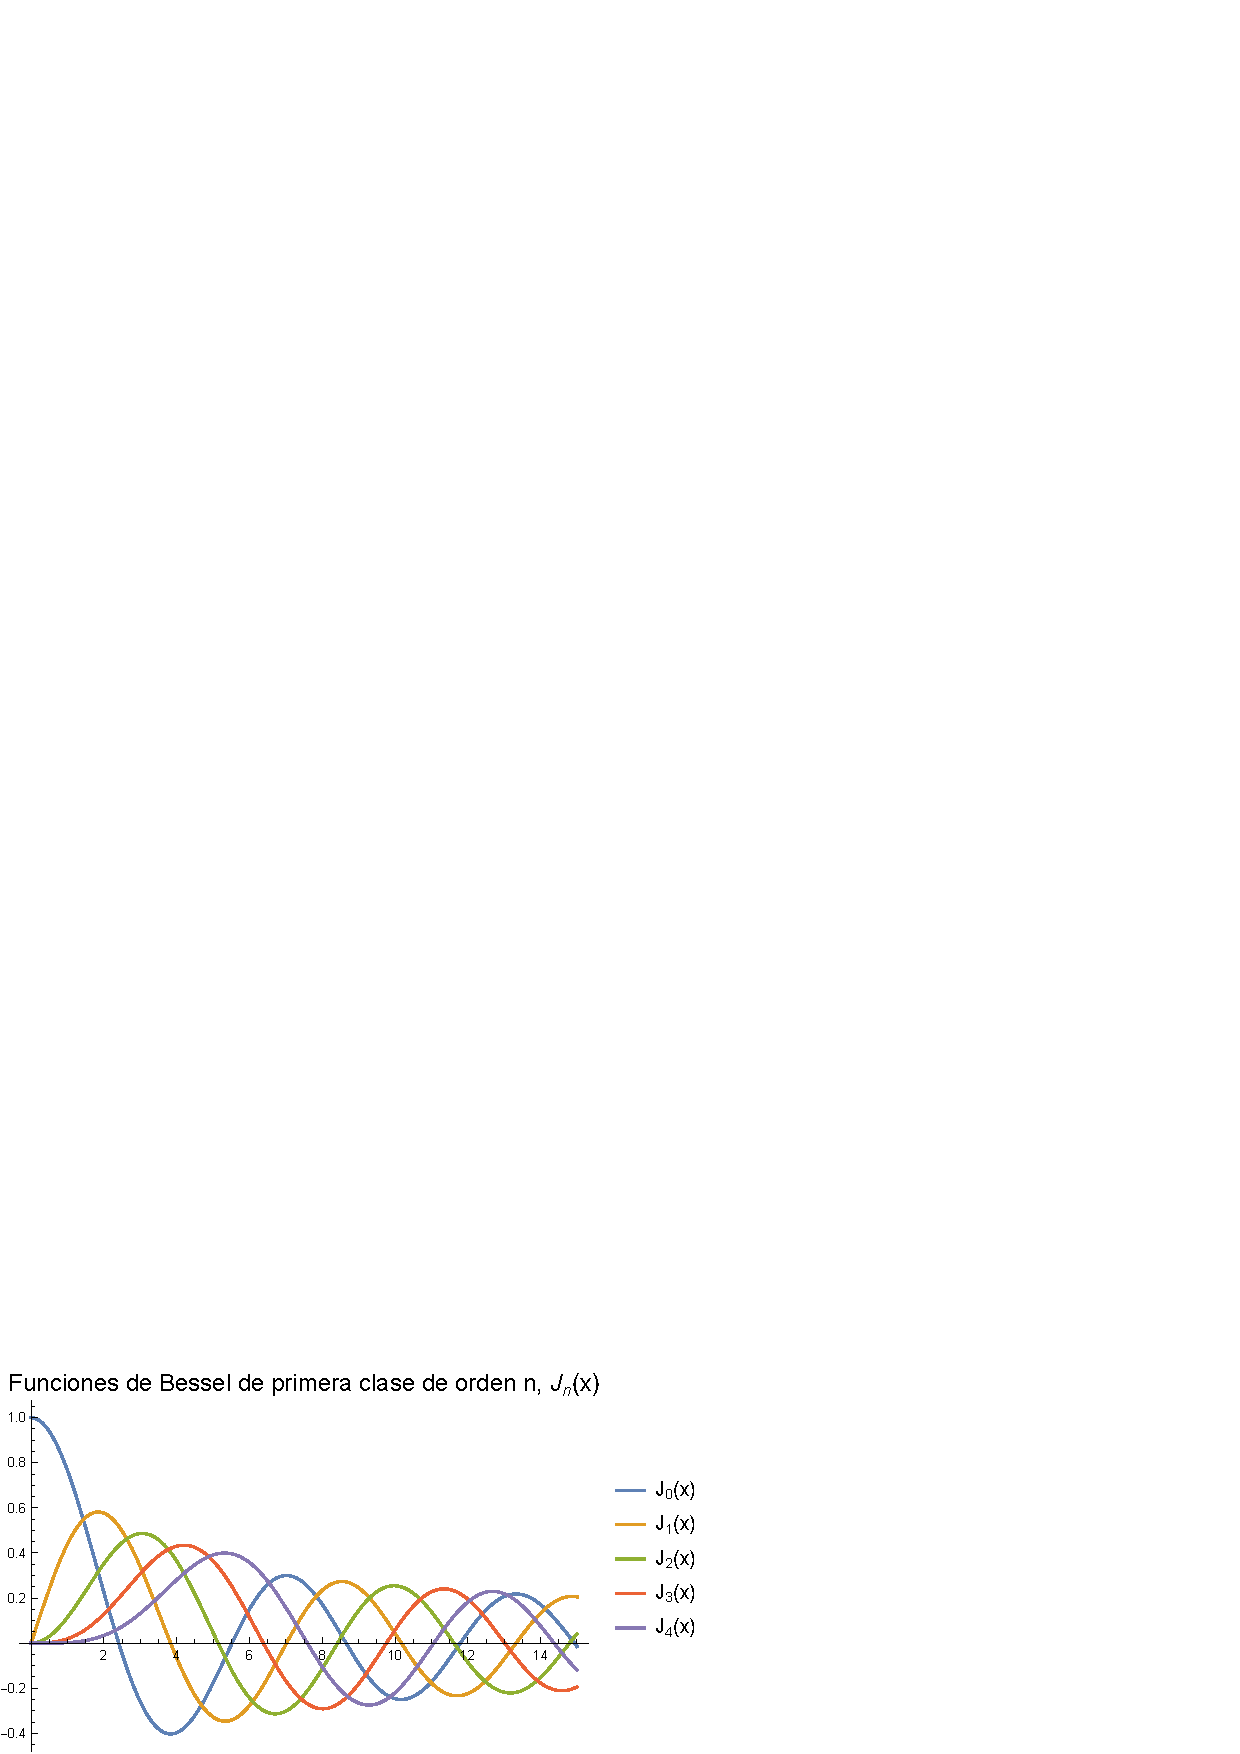
\includegraphics[width=0.9\textwidth]{Imagenes/Plot_Bessel_01_Bessel.pdf}
\end{figure}
\end{frame}
\begin{frame}
\frametitle{Ecuación modificada}
En el caso de que la ecuación de estudio sea de la forma:
\pause
\begin{align*}
\sderivada{R} (r) + \dfrac{1}{r} \, \pderivada{R} (r) + \left( m^{2} - \dfrac{n^{2}}{r^{2}} \right) \, R(r) = 0
\end{align*}
que sería el caso de la ecuación de Laplace, la solución sería una \textocolor{regalia}{función de Bessel modificada}.
\end{frame}
\begin{frame}
\frametitle{Función de Bessel modificada}
A esta función de Bessel modificada, se le conoce también como función de Bessel con argumento imaginario.
\\
\bigskip
\pause
Se le denota como $I_{\nu}(x)$
\end{frame}
\begin{frame}
\frametitle{Función de Bessel modificada}
La función es:
\pause
\begin{align*}
I_{\nu}(x) = \dfrac{x^{\nu}}{2^{\nu} \, \nu!} \left[ 1 + \nsum_{n=1}^{\infty} \dfrac{x^{2n}}{2^{2n} \, n! \, (1 + \nu) \ldots (n + \nu)} \right]
\end{align*}
La función modificada de Bessel se obtiene al sustituir $x$ por $i \, x$ en la ecuación de Bessel.
\end{frame}
\begin{frame}
\frametitle{Las funciones modificadas de Bessel}
\begin{figure}[H]
    \centering
    \includegraphics[width=0.9\textwidth]{Imagenes/Plot_Bessel_02_Bessel_Modificada.pdf}
\end{figure}
\end{frame}
\begin{frame}
\frametitle{Conclusiones}
La ecuación de Bessel es una EDO2, por lo que debería de tener dos soluciones linealmente independientes.
\\
\bigskip
\pause
Haremos de manera conveniente una pausa con la segunda solución, ya que ésta diverge en $x = 0$.
\end{frame}
\begin{frame}
\frametitle{Una regla}
La ecuación mostrada en este ejercicio es de la forma:
\pause
\begin{align*}
\sderivada{y} (r) + \dfrac{d - 1}{r} \, \pderivada{y}(r) + \left( \lambda - \dfrac{\mu}{r^{2}} \right) \, y(r) = 0
\end{align*}
En coord. cilíndricas $d = 2$ y $\mu$ normalmente es $m^{2}$. \pause En coord. esféricas: $d = 3$ y $\mu$ es $k (k + 1)$.
\end{frame}

\subsection{El teorema de Fuchs}

\begin{frame}
\frametitle{El teorema de Fuchs}
El teorema nos dice que se obtendrá al menos una solución en serie de potencias al aplicar el método de Frobenius si el punto de expansión es un punto singular ordinario o regular.
\end{frame}
\begin{frame}
\frametitle{Ejercicio a cuenta}
Para repasar lo que hemos desarrollado hasta el momento, con la siguiente ecuación:
\pause
\begin{align*}
x^{2} \, \sderivada{y} (x) + x \, \pderivada{y} (x) + (x^{2} - 4) \, y (x) = 0
\end{align*}
Determina:
\setbeamercolor{item projected}{bg=carmine,fg=white}
\setbeamertemplate{enumerate items}{%
\usebeamercolor[bg]{item projected}%
\raisebox{1.5pt}{\colorbox{bg}{\color{fg}\footnotesize\insertenumlabel}}%
}
\begin{enumerate}
\item La naturaleza de los puntos singulares.
\item La ecuación de índices.
\seti
\end{enumerate}
\end{frame}
\begin{frame}
\frametitle{Ejercicio a cuenta}
\setbeamercolor{item projected}{bg=carmine,fg=white}
\setbeamertemplate{enumerate items}{%
\usebeamercolor[bg]{item projected}%
\raisebox{1.5pt}{\colorbox{bg}{\color{fg}\footnotesize\insertenumlabel}}%
}
\begin{enumerate}
\conti
\item La regla de recurrencia.
\item La(s) solución(es) en series de potencias.
\end{enumerate}
\end{frame}

\end{document}